\chapter{Implementacija i korisničko sučelje}
		
		
		\section{Korištene tehnologije i alati}
		
			 
			 Za potrebe rada na projektu, tim je komunicirao preko aplikacija WhatsApp\footnote{https://www.whatsapp.com/} i Discord\footnote{https://discord.com/}. 
			 Za izradu UML dijagrama, korišten je alat Astah\footnote{https://astah.net/}.
			 Za upravljanje različitim verzijama datoteka korišten je sustav Git\footnote{https://git-scm.com/}.
			 Udaljeni repozitorij projekta nalazi se na platformi Github\footnote{https://github.com/}. Za izradu i testiranje baze korišten je sustav za upravljanje bazama podataka PostgreSQL\footnote{https://www.postgresql.org/}.
			 
			 Kao integrirano razvojno okruženje (IDE) korišten je Intellij IDEA\footnote{https://www.jetbrains.com/idea/}. Ovaj IDE razvio je JetBrains. Koristi se prvenstveno za razvoj softvera napisanog u Javi, Kotlinu i drugim JVM (Java Virtual Machine) jezicima. Preko pluginova nudi podršku i za mnoge druge programske jezike kao što su Python, R, Julia itd. Za potrebe rada na projektu, tim je koristio studentske licence za navedeni IDE preko kojih je moguće koristiti podršku Intellij-a za razne radne okvire (npr. Spring, React).
			 
			 Aplikacija \textit{Ozdravi} napisana je koristeći radni okvir React\footnote{https://react.dev/} za \textit{frontend} te radni okvir Spring\footnote{https://spring.io} za \textit{backend}.
			 \textit{React} je Javascript biblioteka otvorenog koda za izradu korisničkih sučelja. Održavaju ju Meta i zajednica programera i tvrtki. Ova biblioteka brza je i jednostavna za koristiti te se pomoću nje najčešće razvijaju single-page aplikacije. Velika prednost toga je što React omogućuje da se prilikom korištenja sučelja ponovno naslikaju (renderaju) samo dijelovi koji su se izmijenili. Sučelje izrađeno pomoću Reacta sastavljeno je od komponenti koje se mogu ponovno iskoristiti.
			 \textit{Spring} je besplatan radni okvir za razvoj aplikacija u Javi (i drugim jezicima). Vrlo je popularan zbog različitih modula koje nudi čime se znatno ubrzava stvaranje aplikacije. U sklopu izrade ove aplikacije korišteni su Spring Boot (razvoj aplikacije s minimalnom količinom konfiguracija), Spring Security (jednostavna konfiguracija zaštite aplikacije), Spring Data JPA (za lakšu komunikaciju s bazom podataka) i drugi. Za brzo početno podešavanje korištena je stranica Spring initializr\footnote{https://start.spring.io/}.
				
			
			\eject 
		
	
		\section{Ispitivanje programskog rješenja}
			
	
			
			\subsection{Ispitivanje komponenti}
			Ispitivanje komponenti provedeno je koristeći radni okvir \textit{JUnit 5}. Testovi se u tom radnom okviru pišu jednostavno kao zasebne metode. Ako testna metoda dođe do svog kraja, to znači da je test prošao, a ako se dogodi iznimka, test je pao. Osim toga, \textit{JUnit 5} daje velik broj \textit{assertion} metoda koje provjeravaju dane uvjete i bacaju iznimku (ruše test) ako isti nisu ispunjeni. Ovdje je navedeno 7 testova, od jednostavnijih prema složenijima. \\
			
			\noindent \textbf{Prvi test} [\textit{testFetchNonexistentOsoba}] provjerava baca li se odgovarajuća iznimka pri pokušaju dohvaćanja nepostojeće osobe po OIB-u iz baze podataka. 
			\begin{figure}[H]
				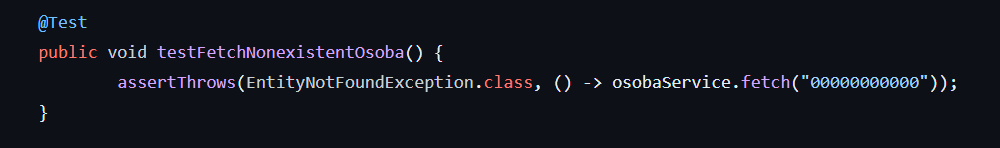
\includegraphics[width=\textwidth]{slike/junit_1.png}
				\caption{Prvi ispitni slučaj}
				\label{fig:junit_1}
			\end{figure}
			% C:\github\Tarantule\dokumentacija\slike
			\noindent \textbf{Drugi test} [\textit{testFetchExistingOsoba}] provjerava dohvaća li se osoba odgovarajućeg imena i prezimena pri dohvaćanju postojeće osobe po OIB-u iz baze podataka.
			\begin{figure}[H]
				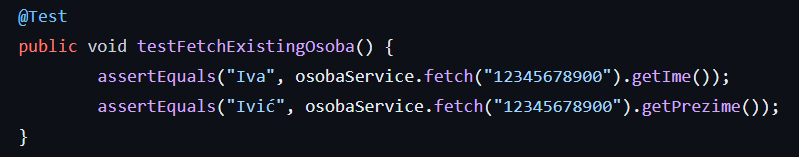
\includegraphics[width=\textwidth]{slike/junit_2.png}
				\caption{Drugi ispitni slučaj}
				\label{fig:junit_2}
			\end{figure}
			
			\noindent \textbf{Treći test} [\textit{testFindOsobaByParentOib}] provjerava funkcionira li metoda za dohvaćanje djece po OIB-u njihovog roditelja na način da usporedi jesu li dobiveni točni OIB-i.
			\begin{figure}[H]
				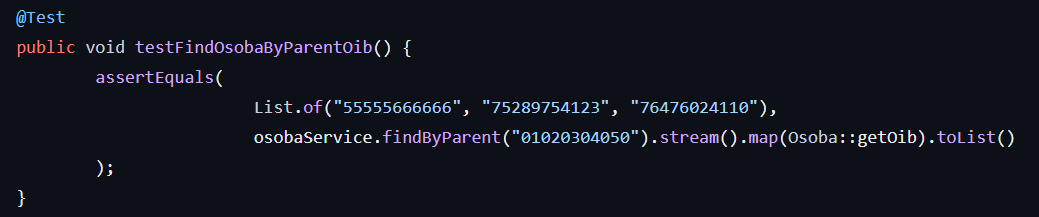
\includegraphics[width=\textwidth]{slike/junit_3.png}
				\caption{Treći ispitni slučaj}
				\label{fig:junit_3}
			\end{figure}
			
			\noindent \textbf{Četvrti test} [\textit{testCreatePoruka}] provjerava može li se dodati validna poruka i hoće li funkcija za stvaranje poruke vratiti dodani objekt.
			\begin{figure}[H]
				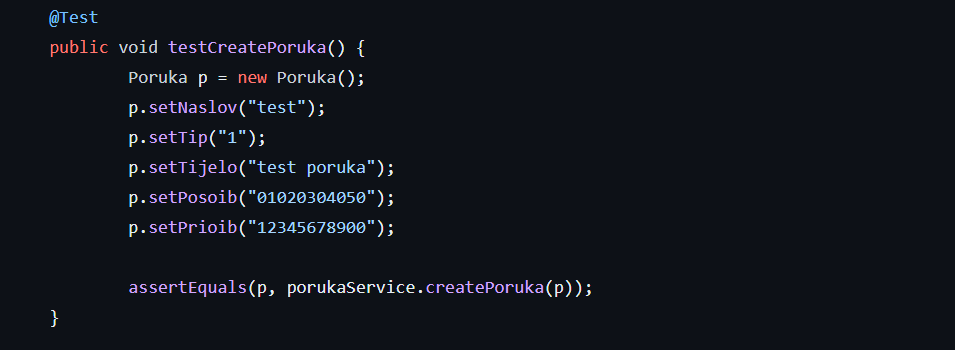
\includegraphics[width=\textwidth]{slike/junit_4.png}
				\caption{Četvrti ispitni slučaj}
				\label{fig:junit_4}
			\end{figure}
			
		 	\noindent \textbf{Peti test} [\textit{testDeletePoruka}] provjerava funkcionira li metoda za brisanje poruke iz baze na način da provjeri vraća li ista objekt s točnim identifikatorom te hoće li nakon toga pokušaj dohvaćanja poruke sa (sada nepostojećim) identifikatorom uzrokovati iznimku jer objekta više nema.
		 	\begin{figure}[H]
		 		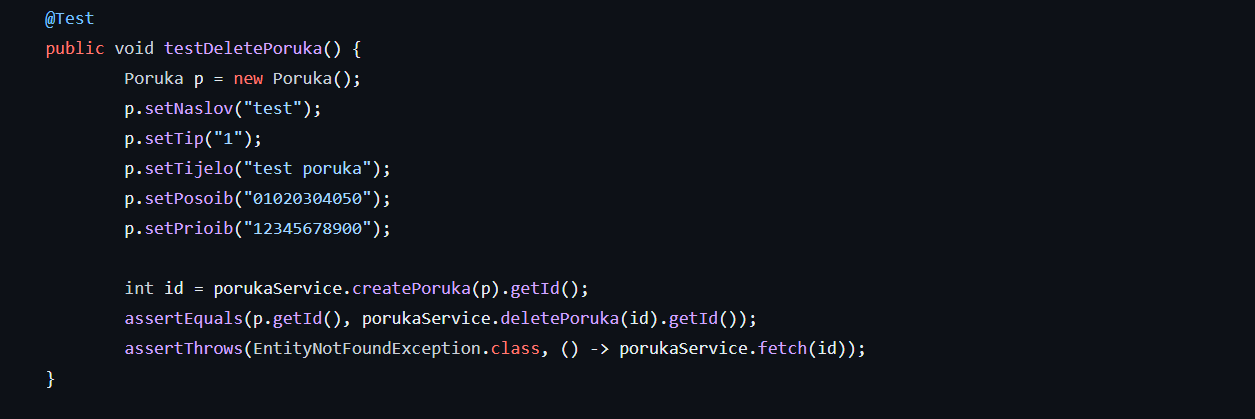
\includegraphics[width=\textwidth]{slike/junit_5.png}
		 		\caption{Peti ispitni slučaj}
		 		\label{fig:junit_5}
		 	\end{figure}
		 	
		 	\noindent \textbf{Šesti test} [\textit{testPorukaBetweenPeople}] provjerava je li moguće ispravno dohvatiti poruke u razgovoru između dvoje ljudi tako da stvori novu poruku između dvoje ljudi i zatim provjeri je li ona među porukama koje vraća testirana metoda. 
		 	\begin{figure}[H]
		 		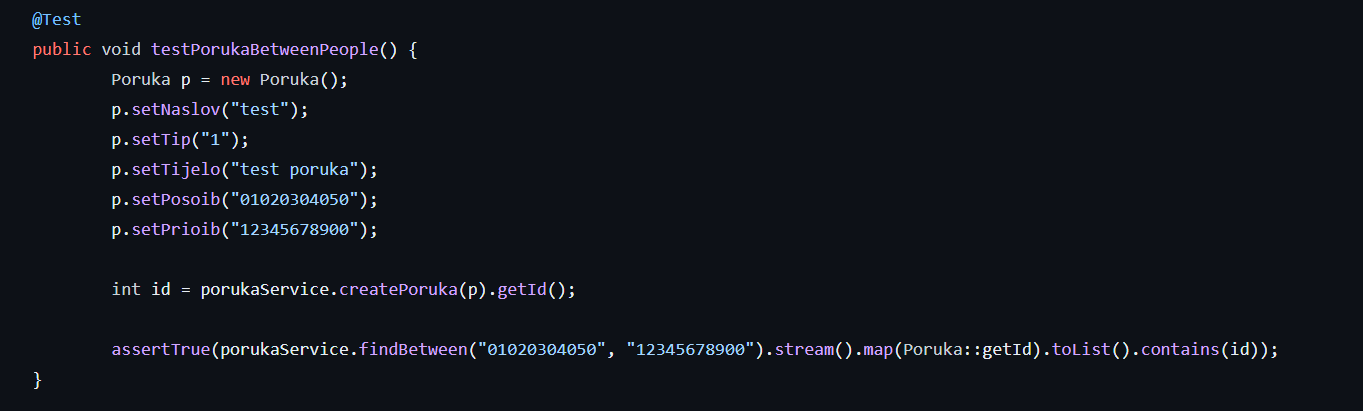
\includegraphics[width=\textwidth]{slike/junit_6.png}
		 		\caption{Šesti ispitni slučaj}
		 		\label{fig:junit_6}
		 	\end{figure}
		 	
		 	\noindent \textbf{Sedmi test} [\textit{testFindUnassignedOsoba}] provjerava metodu koja služi za pronalaženje svih osoba bez doktora/pedijatra. U bazu se doda osoba bez doktora, provjeri se da testirana metoda vraća tu osobu, zatim se osobi doda doktor i konačno se opet poziva testirana metoda i provjeri se da ona ovaj puta ne vraća osobu (jer ona sada ima doktora). 
		 	\begin{figure}[H]
		 		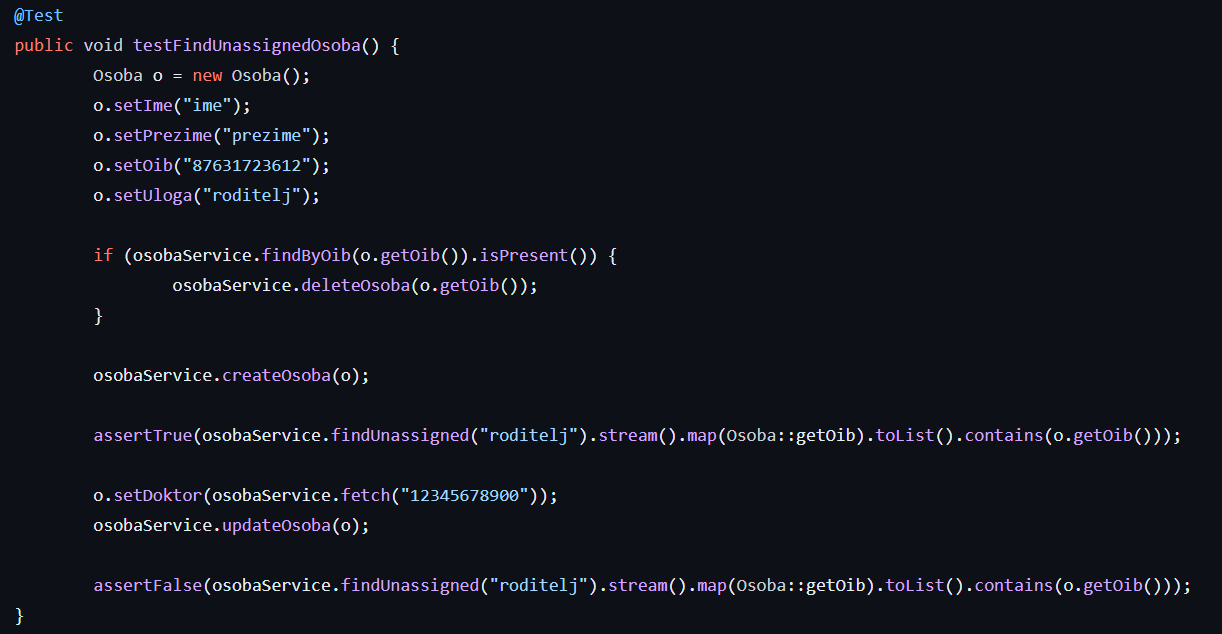
\includegraphics[width=\textwidth]{slike/junit_7.png}
		 		\caption{Sedmi ispitni slučaj}
		 		\label{fig:junit_7}
		 	\end{figure}
		 	
		 	\noindent Konačno, testovi se pokreću pomoću razvojnog okruženja i rezultati su ubrzo vidljivi:
		 	\begin{figure}[H]
		 		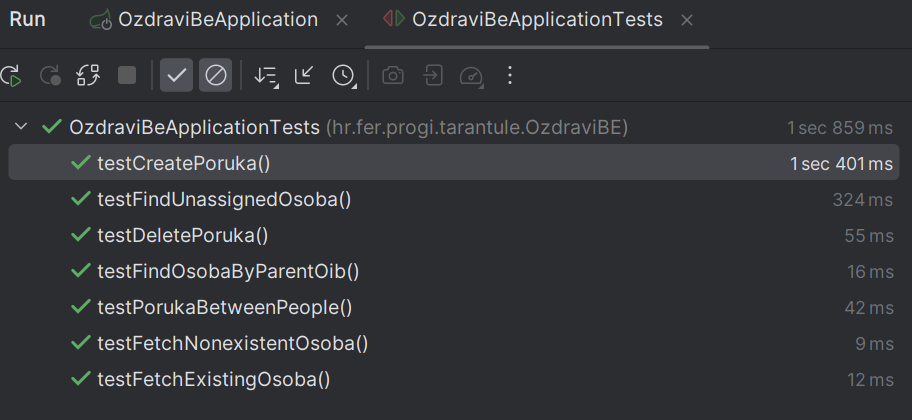
\includegraphics[width=\textwidth]{slike/junit_result.png}
		 		\caption{Rezultati testova}
		 		\label{fig:junit_result}
		 	\end{figure}
			
			\subsection{Ispitivanje sustava}
			
			Testovi su izvršeni pomoću Selenium IDE ekstenzije za Google Chrome. Selenium IDE omogućava automatsko testiranje funkcionalnosti web stranica. Ovaj pristup olakšava identifikaciju grešaka i poboljšava efikasnost procesa testiranja, pružajući preciznost i brzinu u otkrivanju potencijalnih problema.\\ 
				Sam proces testiranja sastoji se od snimanja korisnikovih akcija koje se zatim spremaju kao test. Svaki test moguće je višetruko pokretat te mijenjat unesene parametre. U dokumentaciji je prikazano i opisano testiranje četiri osnovna obrasca uporabe (UC2, UC7, UC24, UC5).\\
			
			\noindent \textbf{Prvi test} provjerava proces prijave u sustav već registriranog korisnika (UC2 - Prijavi se). Tijek testiranja:\\
			Ulazi: 
			\begin{enumerate}
				\item Otvaranje web stranice u pregledniku.
				\item Pritisak na gumb „Prijava“.
				\item Pritisak polja „oib“.
				\item Unos OIB-a postojećeg korisnika.
				\item Pritisak polja „password“
				\item Unos lozinke postojećeg korisnika.
				\item Pritisak na gumb „prijava“.
			\end{enumerate}
			
			\noindent Očekivani rezultat: prikaz stranice korisničkog profila.\\
			Rezultat: očekivani rezultat je zadovoljen i aplikacija prolazi test.
			
			\begin{figure}[H]
				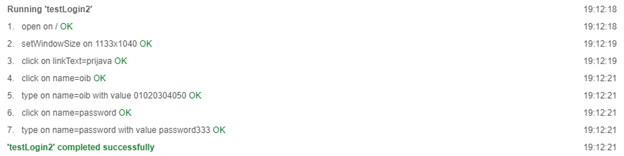
\includegraphics[width=\textwidth]{slike/prijavaUSustav.PNG} %veličina u odnosu na širinu linije
				\caption{Rezultati prvog ispitnog slučaja}
				\label{fig:prijavaTest} %label mora biti drugaciji za svaku sliku
			\end{figure}
			\eject 
		
		\noindent \textbf{Drugi test} provjerava pregled podataka o naručenom specijalističkom pregledu (UC7). \\
			Ulazi: 
		\begin{enumerate}
			\item Odabir profila.
			\item Odabir poruke s naslovom "Naručen pregled".
			\item Pritisak kursorom na kartu, pomicanje kotačića na mišu.
			\item Pritisak kursorom na jednu od označenih bolnica.
		\end{enumerate}
		
		\noindent Očekivani rezultati:\\ Prikazuje se karta sa svim bolnicama iz baze podataka koje su u blizni stanovanja pacijenta. Na karti je moguće mijenjati visinu i poziciju pogleda te otvoriti ikonu s nazivom bolnice.\\
		Rezultati: očekivani rezultat je zadovoljen i aplikacija prolazi test.
		
		\begin{figure}[H]
			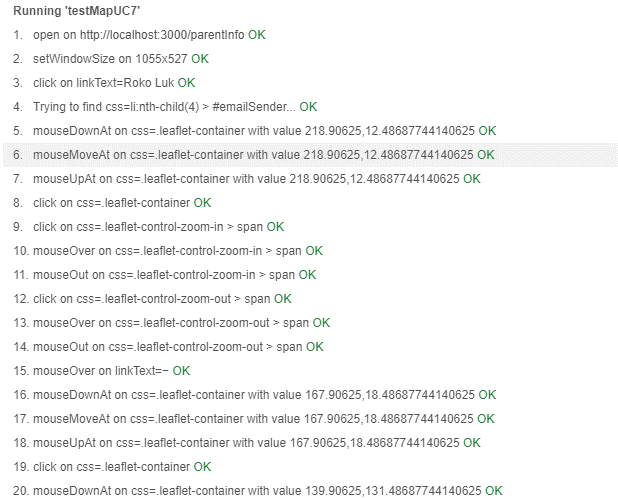
\includegraphics[width=\textwidth]{slike/pregledNaručivanja.PNG} %veličina u odnosu na širinu linije
			\caption{Rezultati drugog ispitnog slučaja}
			\label{fig:pregledKarteTest} %label mora biti drugaciji za svaku sliku
		\end{figure}
		\begin{figure}[H]
			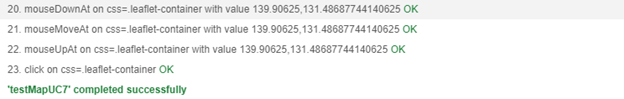
\includegraphics[width=\textwidth]{slike/pregledNaručivanja2.PNG} %veličina u odnosu na širinu linije
			\caption{Rezultati drugog ispitnog slučaja}
			\label{fig:pregledKarteTest2} %label mora biti drugaciji za svaku sliku
		\end{figure}
		
		
		\noindent \textbf{Treći test} provjerava akciju propisivanja bolovanja roditelju (UC24).\\
		Ulazi:
		\begin{enumerate}
			\item Odabir profila roditelja.
			\item Pritisak na „Nova poruka.
			\item Unos teksta poruke.
			\item Označavanje opcije „Bolovanje roditelja“.
			\item Pritisak gumba "Pošalji".
		\end{enumerate}
		Očekivani rezultati:\\Prikaz profila roditelja s novom porukom naziva "dijagnoza". Odabirom te poruke prikazuje se prikaz za čitanje poruke u kojoj vidimo sadržaj i na dnu tekst „Odobreno bolovanje“.\\
		Rezultat: Očekivani rezultat je zadovoljen. Aplikacija je prošla test.
		
		\begin{figure}[H]
			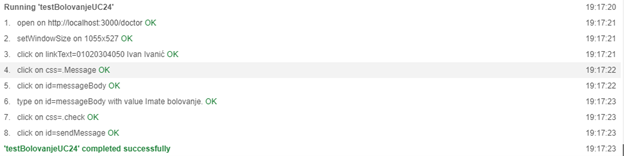
\includegraphics[width=\textwidth]{slike/propisivanjeBolovanja.PNG} %veličina u odnosu na širinu linije
			\caption{Rezultati trećeg ispitnog slučaja}
			\label{fig:propisivanjeBolovanjaTest} %label mora biti drugaciji za svaku sliku
		\end{figure}
		\eject 
		
		\noindent \textbf{Četvrti test} provjerava izmjenu osobnih podataka na stranici roditelja/djeteta (UC 5).\\
		Ulazi:
		\begin{enumerate}
			\item Odabir profila roditelja/djeteta.
			\item Pritisak ikone za izmjenu podataka.
			\item Odabir polja za izmjenu.
			\item Unos novih podataka.
			\item Pritisak na gumb "spremi.
		\end{enumerate}
		Očekivani rezultati:\\ Prikazuje se stranica korisničkog profila. Po otvaranju prozora s osobnim podatcima prikazuju se ažurirani podatci.\\
		Rezultati: Očekivani rezultat je zadovoljen. Aplikacija je prošla test.
		
		\begin{figure}[H]
			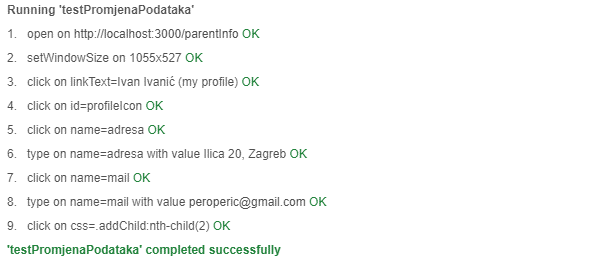
\includegraphics[width=\textwidth]{slike/promjenaPodataka.PNG} %veličina u odnosu na širinu linije
			\caption{Rezultati četvrtog ispitnog slučaja}
			\label{fig:promjenaPodatakaTest} %label mora biti drugaciji za svaku sliku
		\end{figure}
		\eject
		
		Poslijednjim testom prikazujemo kako sustav reagira ukoliko test ne prolazi. Test je proveden ponovnim pokretanjem prvog testa, no ovaj put s neispravnom lozinkom. Očekivani izlaz je neuspješna prijava korisnika te prikaz poruke o pogrešci.
		
		\begin{figure}[H]
			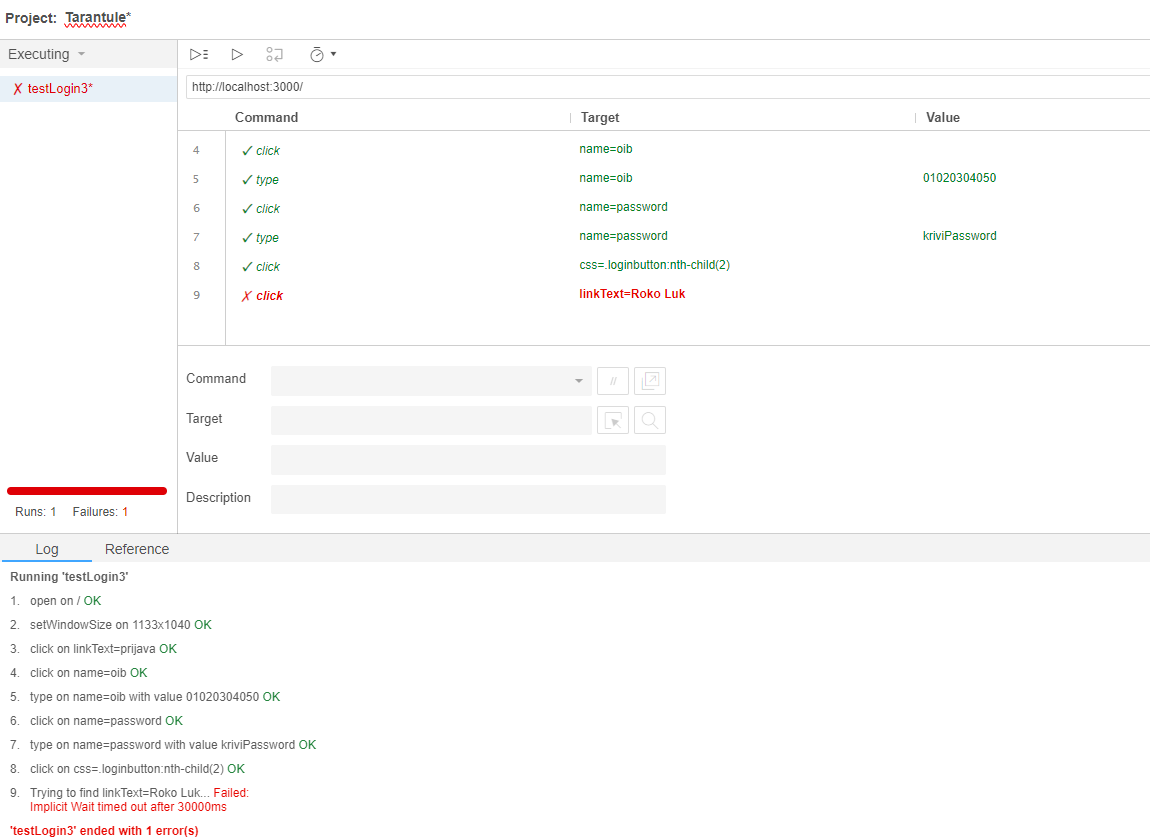
\includegraphics[width=\textwidth]{slike/neispravnaPrijava.PNG} %veličina u odnosu na širinu linije
			\caption{Rezultati i parametri petog ispitnog slučaja}
			\label{fig:neispravnaPrijavaTest} %label mora biti drugaciji za svaku sliku
		\end{figure}
		\eject
		
		\section{Dijagram razmještaja}
			
			 
			 Dijagram razmještaja je strukturni UML dijagram koji opisuje topologiju sustava i prikazuje odnos sklopovskih i programskih dijelova. Na slici \ref{fig:dijagramrazmjestaja} prikazan je specifikacijski dijagram razmještaja aplikacije. Na čvoru koji predstavlja korisnički uređaj nalazi se web preglednik (artefakt) korisnika. On preko HTTPS protoka komunicira s poslužiteljem. Poslužitelj pruža uslugu poslužitelja frontenda, backenda te baze podataka. Sve te usluge mogu međusobno komunicirati slanjem zahtjeva.
			 
			 \begin{figure}[H]
			 	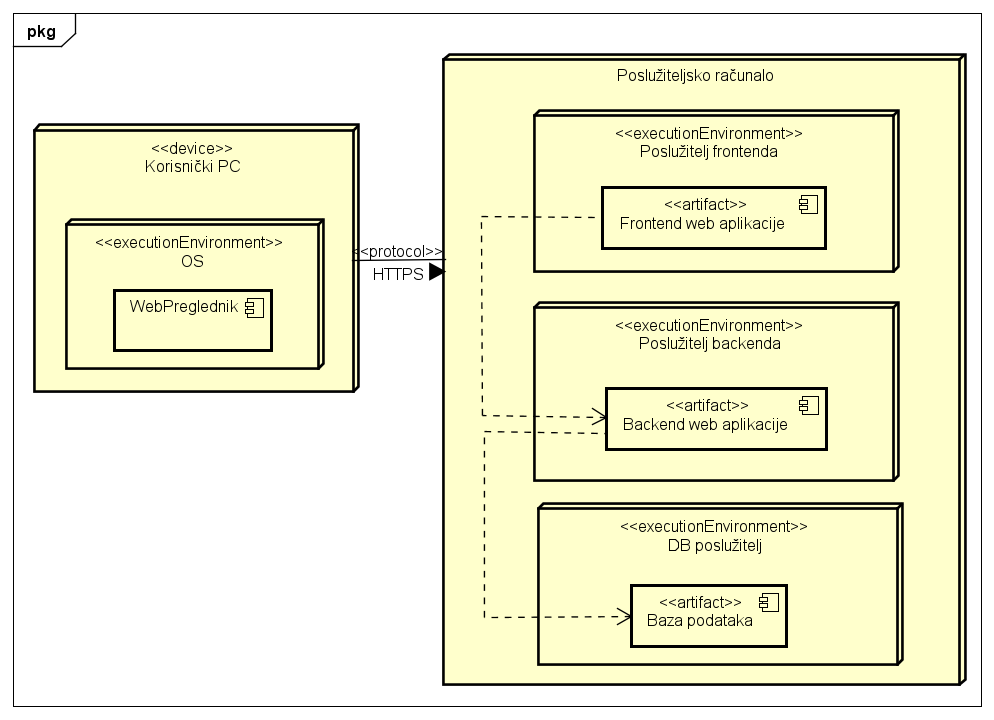
\includegraphics[width=\textwidth]{dijagrami/Dijagram razmjestaja.PNG} %veličina u odnosu na širinu linije
			 	\caption{Dijagram razmještaja}
			 	\label{fig:dijagramrazmjestaja} %label mora biti drugaciji za svaku sliku
			 \end{figure}
			
			\eject 
		
		\section{Upute za puštanje u pogon}
			 
			 Za deploy aplikacije se koristi servis Render\footnote{https://render.com/} koji nudi opciju korištenja besplatnih instanci na cloudu. Naravno, one nude malo procesorske snage i također imaju neka druga ograničenja ali je to sasvim dovoljno za ovaj projekt. Potrebno je napraviti tri instance na Renderu: na jednoj će biti upogonjen backend, druga ce posluživati frontend, a treća PostgreSQL bazu podataka.
			 
			 
			 \textbf{Backend}
			 
			 Napraviti instancu tipa “web service”. Povezati ju s git repozitorijem u kojemu se nalazi projekt. Ime odabrati proizvoljno (ovdje \textit{ozdraviapp-be}), regiju postaviti na geografski najbližu (Frankfurt), za granu izabrati master, a za korijenski direktorij onaj u kojemu se nalazi Java projekt za backend. Konačno, runtime će biti Docker, a zbog toga je potrebno napraviti još nekoliko koraka prije nego se aplikacija može deployati.
			 
			 Kako bi se Docker mogao koristiti pri deployu, potrebno je u korijenski direktorij backend projekta dodati novi direktorij \textit{docker} i u njemu Dockerfile. Njegov sadržaj vidljiv je na slici \ref{fig:docker1}.
			 
			 \begin{figure}[H]
			 	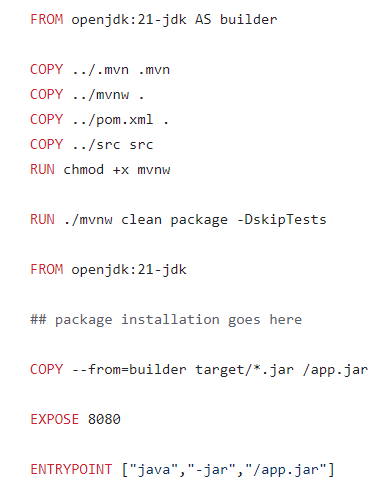
\includegraphics[width=\textwidth]{slike/docker.PNG} %veličina u odnosu na širinu linije
			 	\caption{Dockerfile}
			 	\label{fig:docker1} %label mora biti drugaciji za svaku sliku
			 \end{figure}
			 
			 Ukratko, Dockerfile će napraviti okruženje u koje će kopirati izvorni kod backenda i sve potrebne datoteke te kompajlirati taj kod, a zatim u drugo okruženje kopirati dobiveni \textit{.jar}. Na kraju, definira se da se pri pokretanju kontejnera pokreće upravo taj \textit{.jar} pomoću JVM. Koriste se Docker slike openjdk:21-jdk, zbog toga što je potreban JDK kako bi se kompajlirao Java projekt.
			 
			 Sada se na Renderu može izabrati besplatna verzija instance te stvoriti web servis. Potrebno je namjestiti varijable okruženja, što se može pronaći u kartici “Environment”.
			 
			 Spring za spajanje na bazu podataka koristi varijable \textit{SPRING\_DATASOURCE\_URL}, \textit{SPRING\_DATASOURCE\_NAME}, \textit{SPRING\_DATASOURCE\_PASSWORD}. Sve one moraju biti postavljene na odgovarajuće vrijednosti kako bi aplikacija funkcionirala. Ove varijable se mogu definirati tek kad se stvori Render instanca za posluživanje baze podataka.
			 
			 Na kraju, servis se pokreće klikom na opciju “manual deploy - deploy latest commit”, no ovo se treba napraviti tek nakon namještanja baze podataka.
			 
			 \begin{figure}[H]
				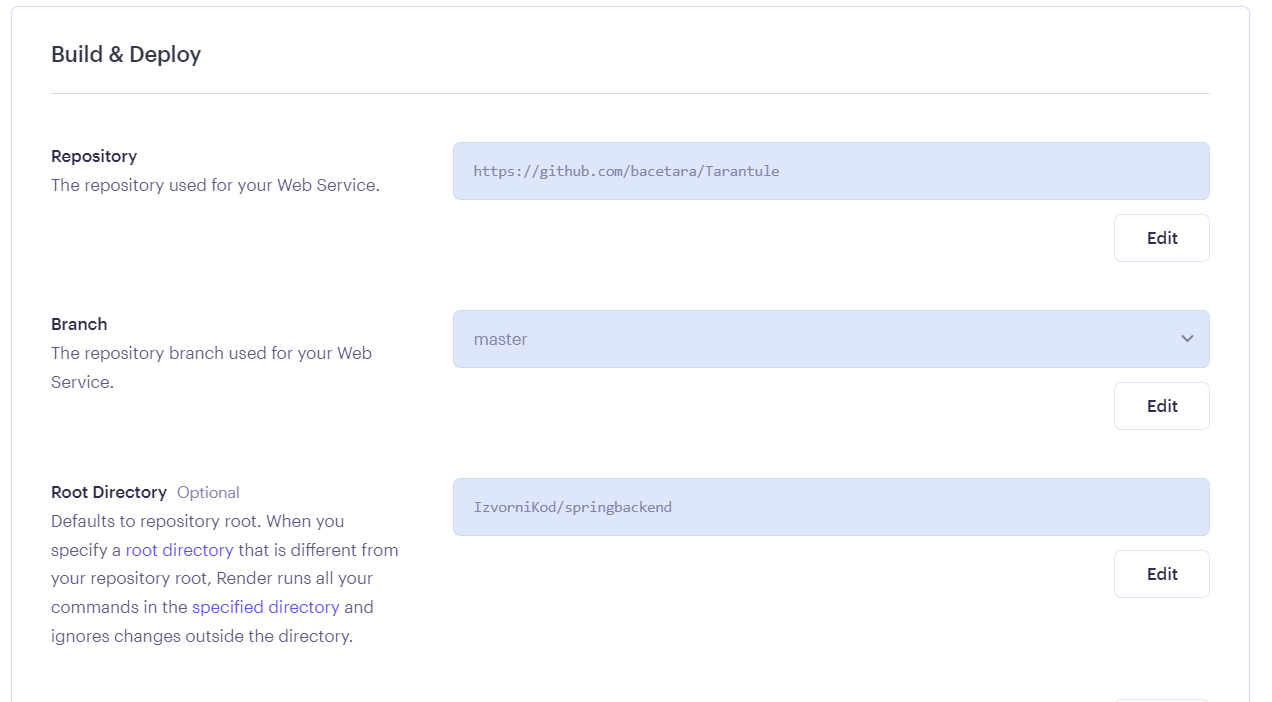
\includegraphics[width=\textwidth]{slike/beDeploy1.png} %veličina u odnosu na širinu linije
				\caption{Postavke za backend instancu, prvi dio}
				\label{fig:beDeploy1} %label mora biti drugaciji za svaku sliku
			 \end{figure}

			 \begin{figure}[H]
				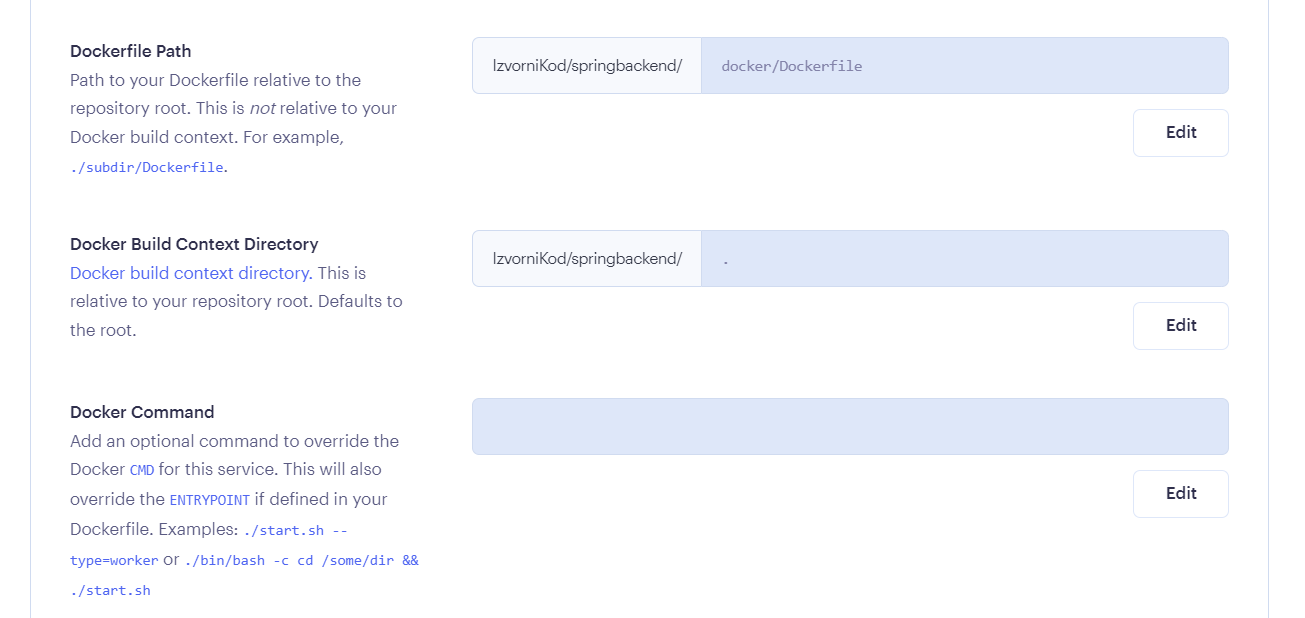
\includegraphics[width=\textwidth]{slike/beDeploy2.png} %veličina u odnosu na širinu linije
				\caption{Postavke za backend instancu, drugi dio}
				\label{fig:beDeploy2} %label mora biti drugaciji za svaku sliku
			 \end{figure}

			 \begin{figure}[H]
				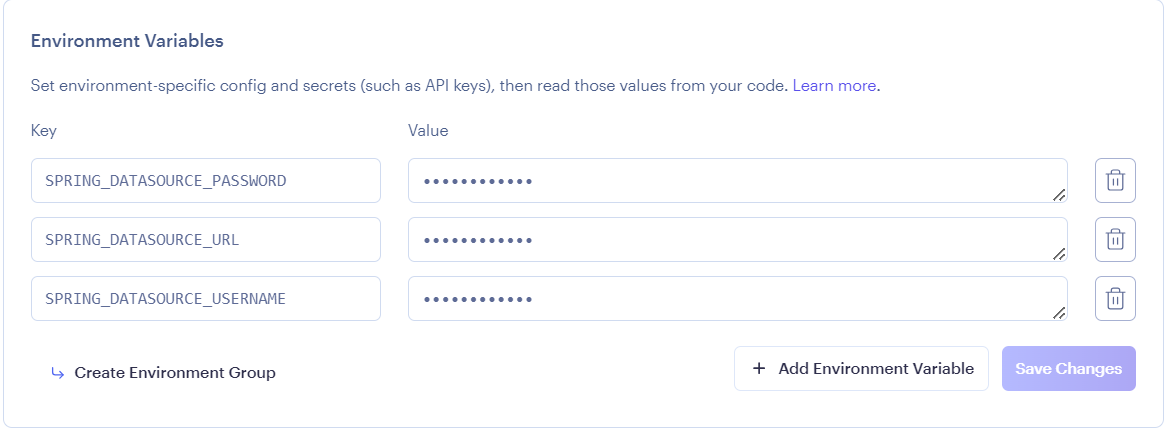
\includegraphics[width=\textwidth]{slike/environmentBe.png} %veličina u odnosu na širinu linije
				\caption{Varijable okruženja za backend}
				\label{fig:beEnv} %label mora biti drugaciji za svaku sliku
			 \end{figure}
			 
			 \textbf{Baza podataka}
			 
			 Napraviti instancu tipa “PostgreSQL”. Za regiju odabrati opet geografski najbližu, a imena instance, baze i korisnika izabrati proizvoljno. Uzeti besplatnu opciju i kreirati instancu.
			 
			 U postavkama instance se sada može pronaći URL baze podataka na poslužitelju, kao i lozinka za kreiranog korisnika. Ove podatke valja zapisati u odgovarajuće varijable okruženja u instanci za backend. Osim toga, prikazana je i naredba koja se može iskoristiti za povezivanje na bazu podataka. Sada je dovoljno iskoristiti tu naredbu za spajanje na bazu podataka i dalje je sve isto kao i kad se radi lokalno. Sa “\textbackslash i  \textit{imeSqlSkripte}” se može pokrenuti skripta za stvaranje tablica i sl.
			 
			 Pri radu s bazom podataka treba obratiti pozornost na kodne stranice. Zato je važno (vrijedi za Windows okruženje) prije spajanja na bazu podataka unijeti naredbu “\textit{chcp 65001}”, a nakon spajanja na bazu unijeti SQL naredbu “\textit{set client\_encoding = ‘UTF8’}”, kako bi se hrvatska slova ispravno prikazivala.
			 
			 \begin{figure}[H]
				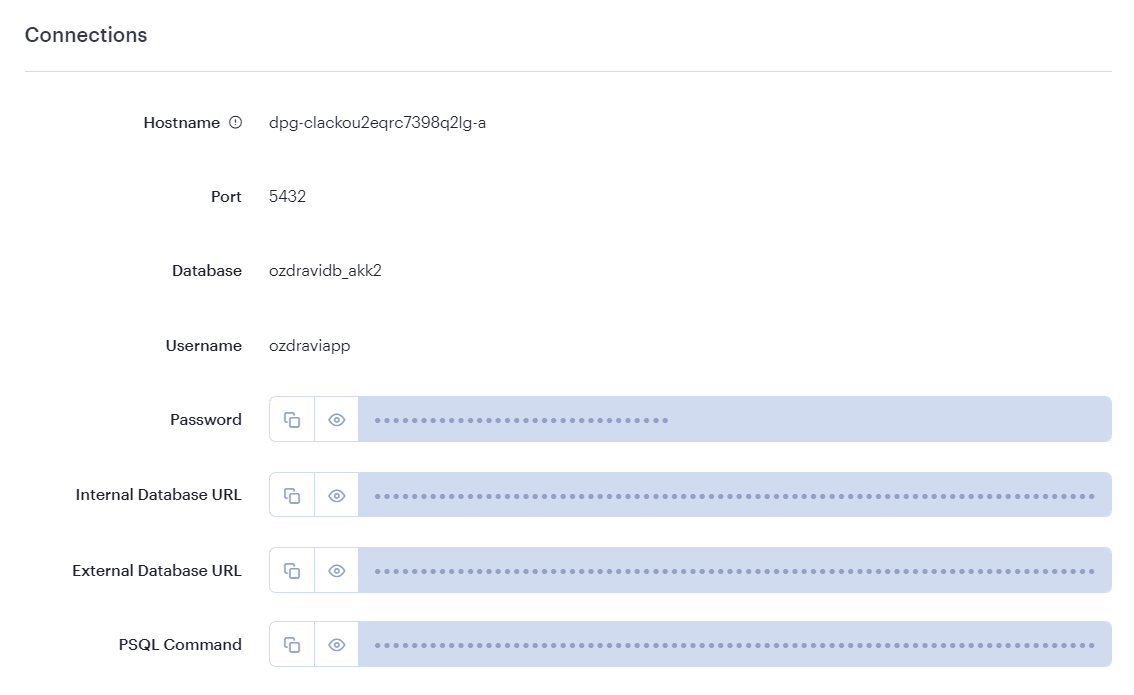
\includegraphics[width=\textwidth]{slike/bazaDeploy.png} %veličina u odnosu na širinu linije
				\caption{Postavke za instancu baze podataka}
				\label{fig:bazaDeploy} %label mora biti drugaciji za svaku sliku
			 \end{figure}
			 
			 \textbf{Frontend}
			 
			 Opet, stvoriti Render instancu, ovog puta tipa “web servis”, kao i za backend. Povezati s git repozitorijem. Postavke izabrati na analogan način kao i za backend. Ime proizvoljno (ovdje \textit{ozdraviapp-fe}), regija geografski najbliža, grana master, korijenski direktorij frontend projekta i besplatna verzija. No, ovdje runtime neće biti Docker već Node.js. U polje \textit{Build command} upisati "\textit{yarn build}", a u polje \textit{Start command} upisati "\textit{npm start}".
			 
			 Kako bi frontend funkcionirao, treba mu dati do znanja gdje se nalazi backend. To treba postaviti u datoteci setupProxy.js. Za lokalno testiranje, postavljeno je da svi pozivi prema putanjama /api/… budu preusmjereni na localhost:8080 (port na kojemu je backend). Analogno tome, za deploy ovi pozivi trebaju ići na URL na kojemu se nalazi backend (npr. \textit{ozdraviapp-be.onrender.com}), a koji se može pronaći u postavkama instance na kojoj je backend.
			 Taj se URL može ili kodirati u samu datoteku setupProxy.js ili postaviti kao varijabla okruženja na render instanci za frontend (što je bolja opcija) i onda se u kodu dohvatiti pomoću “process.env.IME\_VARIJABLE”. Sada se frontend može pokrenuti na isti način kao i backend, opcijom “manual deploy - deploy latest commit”.
			 
			 Aplikaciji se sada može pristupiti koristeći URL frontenda (\href{ozdraviapp-fe.onrender.com}{što se tiče ove aplikacije ovdje}). Valja napomenuti da se nakon perioda nekorištenja render instance same gase, pa je zato prvo pokretanje nakon nekoliko sati obično vrlo sporo.
			
			 \begin{figure}[H]
				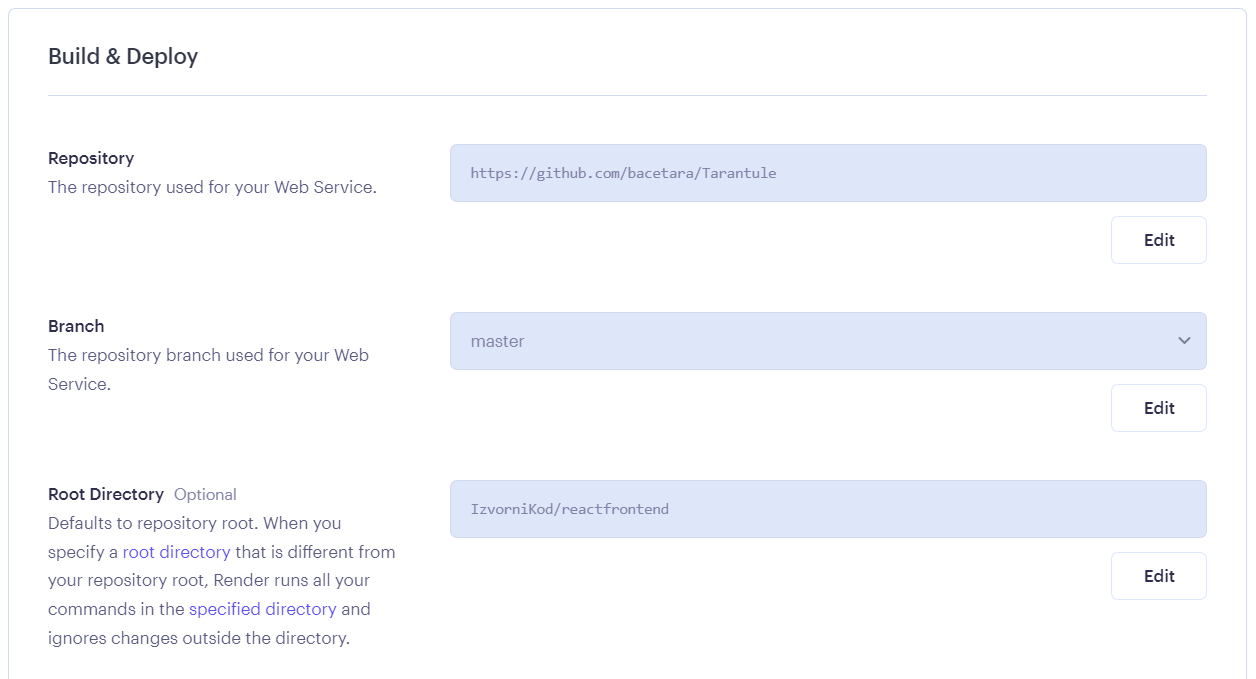
\includegraphics[width=\textwidth]{slike/feDeploy1.png} %veličina u odnosu na širinu linije
				\caption{Postavke za frontend instancu, prvi dio}
				\label{fig:feDeploy1} %label mora biti drugaciji za svaku sliku
			 \end{figure}

			 \begin{figure}[H]
				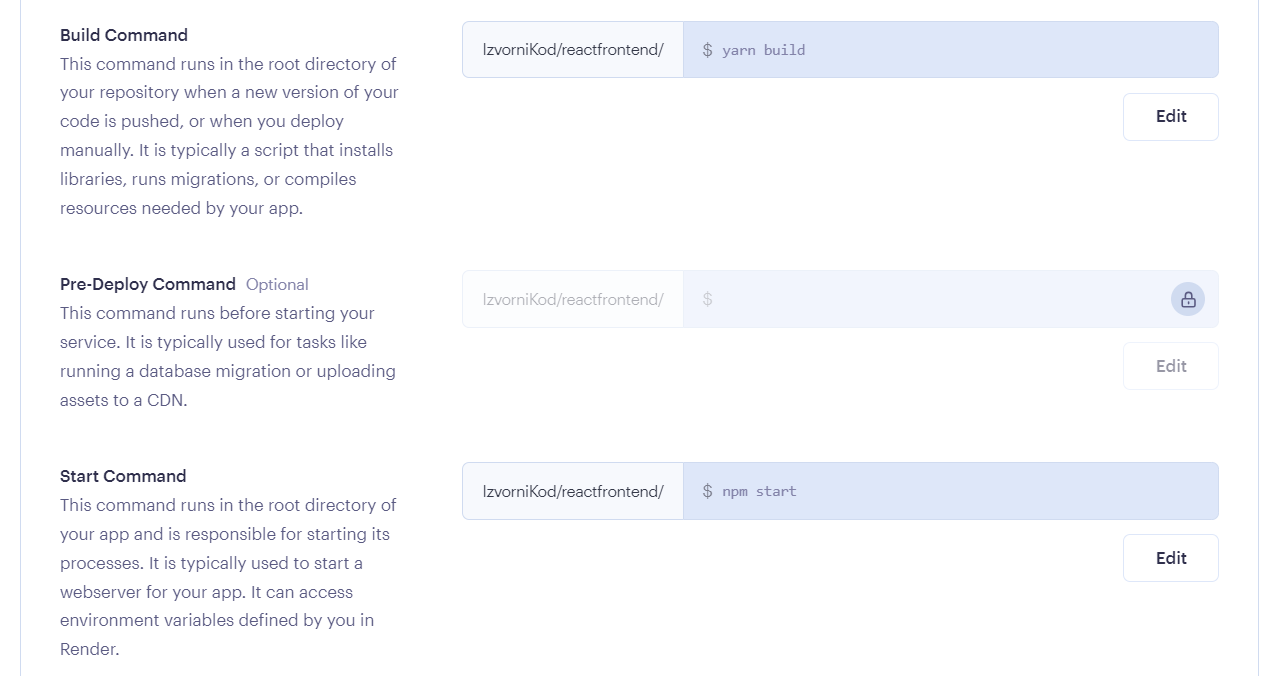
\includegraphics[width=\textwidth]{slike/feDeploy2.png} %veličina u odnosu na širinu linije
				\caption{Postavke za frontend instancu, drugi dio}
				\label{fig:feDeploy2} %label mora biti drugaciji za svaku sliku
			 \end{figure}
			 
			 \begin{figure}[H]
				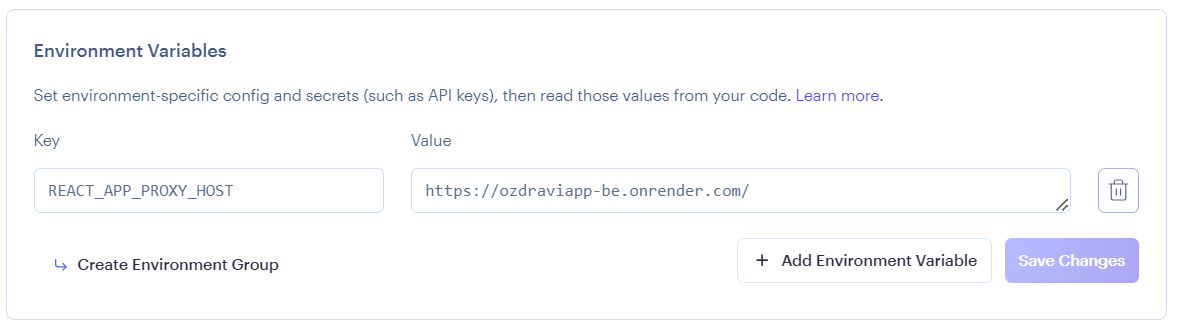
\includegraphics[width=\textwidth]{slike/environmentFe.png} %veličina u odnosu na širinu linije
				\caption{Varijable okruženja za frontend}
				\label{fig:environmentFe} %label mora biti drugaciji za svaku sliku
			 \end{figure}
			
			
			\eject 